% !TEX root = ../../../main.tex

\toggletrue{image}
\toggletrue{imagehover}
\chapterimage{pointers}
\chapterimagetitle{\uppercase{Pointers}}
\chapterimageurl{https://xkcd.com/138/}
\chapterimagehover{Every computer, at the unreachable memory address 0x-1, stores a secret. I found it, and it is that all humans ar—SEGMENTATION FAULT}

\chapter{Hexadezimalcode}
\label{chapter-hexadezimalcode}

Der Hexadezimalcode wird in der Informatik gerne verwendet, da wir somit Dualzahlen kompakter darstellen können. Der Code wird zum Beispiel bei den Unicode Code Points eingesetzt (siehe \autoref{chapter-textcodierungen}) oder bei der Angabe von Farben am Computer (etwa in einem Bildbearbeitungsprogramm wie Adobe Photoshop).

\newcommand{\hexadezimalcodeLernziele}{
\protect\begin{todolist}
\item Sie erklären an einem Beispiel, wie der Hexadezimalcode aufgebaut ist.
\item Sie wandeln eine gegebene Dualzahl in die entsprechende Hexadezimalzahl um.
\item Sie wandeln eine gegebene Hexadezimalzahl in die entsprechende Dualzahl um.
\item Sie wandeln eine gegebene Dezimalzahl in die entsprechende Hexadezimalzahl um.
\item Sie wandeln eine gegebene Hexadezimalzahl in die entsprechende Dezimalzahl um.
\end{todolist}
}

\lernziel{\autoref{chapter-hexadezimalcode}, \nameref{chapter-hexadezimalcode}}{\protect\hexadezimalcodeLernziele}

\hexadezimalcodeLernziele

\section{Zeichen des Hexadezimalcodes}

Der Hexadezimalcode (kurz Hexcode) funktioniert im Prinzip gleich wie das Dezimalsystem oder der Dualcode. Wir benötigen für den Hexadezimalcode sechzehn verschiedene Zeichen. Wir verwenden die üblichen Ziffern des Dezimalsystems ($0$ bis $9$) und fügen noch sechs Buchstaben ($A$, $B$, $C$, $D$, $E$ und $F$) hinzu. Damit können wir dann \textbf{sechzehn verschiedene Zeichen}\footnote{Deshalb auch der Name: Hexa für sechs und Dezimal für 10, d.h. Hexadezimal steht für 16.} mit einer Stelle darstellen (siehe \autoref{table-hex}).

\begin{table}[htb]
\centering
\begin{tabular}{|r|r|r||r|r|r|}
\hline
Hex & Dual & Dez & Hex & Dual & Dez \\ \hline
0 & 0000 & 0 & 8 & 1000 & 8 \\ \hline
1 & 0001 & 1 & 9 & 1001 & 9 \\ \hline
2 & 0010 & 2 & A & 1010 & 10 \\ \hline
3 & 0011 & 3 & B & 1011 & 11 \\ \hline
4 & 0100 & 4 & C & 1100 & 12 \\ \hline
5 & 0101 & 5 & D & 1101 & 13 \\ \hline
6 & 0110 & 6 & E & 1110 & 14 \\ \hline
7 & 0111 & 7 & F & 1111 & 15 \\ \hline
\end{tabular}
\caption{Es ist auch üblich die Kleinbuchstaben $a$ bis $f$ zu verwenden.}
\label{table-hex}
\end{table}

Ein Hexadezimalzeichen deckt \qty{4}{\bit} ab. \autoref{table-hex} zeigt für jedes Hexadezimalzeichen die passende Codierung. Die Spalte \say{Dual} zeigt die Codierung zur Dualzahl. Die Spalte \say{Dez} die Codierung zur Dezimalzahl.

\section{Wo wird der Hexcode eingesetzt?}

\begin{example}[Siebensegmentanzeige]
Bei einer Segmentanzeige\footnote{\url{https://de.wikipedia.org/wiki/Segmentanzeige}}, wie sie bei Digitaluhren oder Taschenrechnern gerne verbaut werden, können durch den Hexcode mit einem Anzeigeelement sechzehn verschiedene Zahlen dargestellt werden (siehe \autoref{figure-siebensegmentanzeige}). Auch der Unicode verwendet den Hexcode zur Darstellung der Code Points.
\end{example}

\begin{figure}[htb]
\centering
\begin{minipage}{0.45\textwidth}
\centering
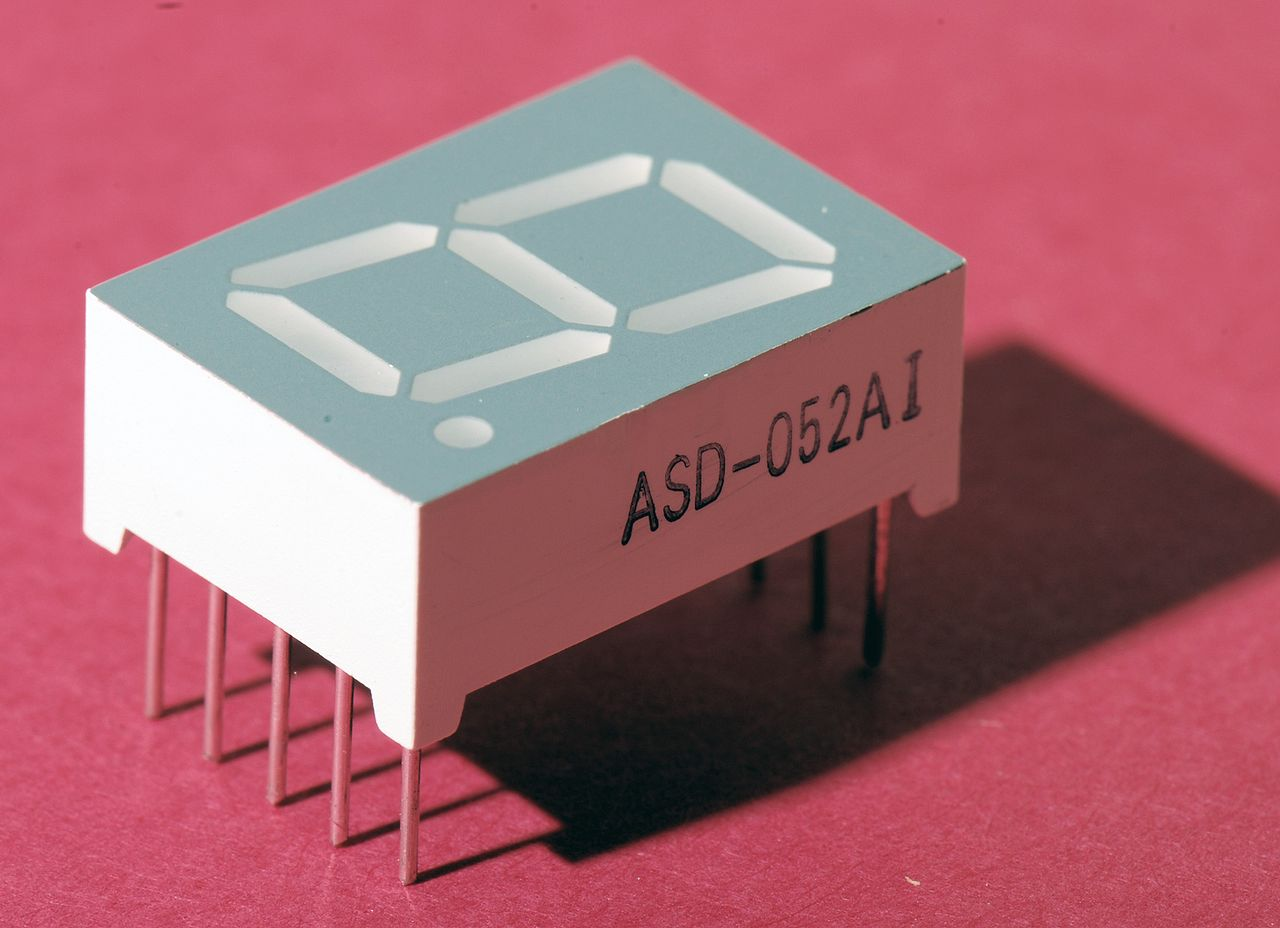
\includegraphics[height=2cm]{siebensegmentanzeige}
\caption{Siebensegmentanzeige. Es können sieben Balken leuchten.}
\label{figure-siebensegmentanzeige}
\end{minipage}
\hfill
\begin{minipage}{0.45\textwidth}
\centering
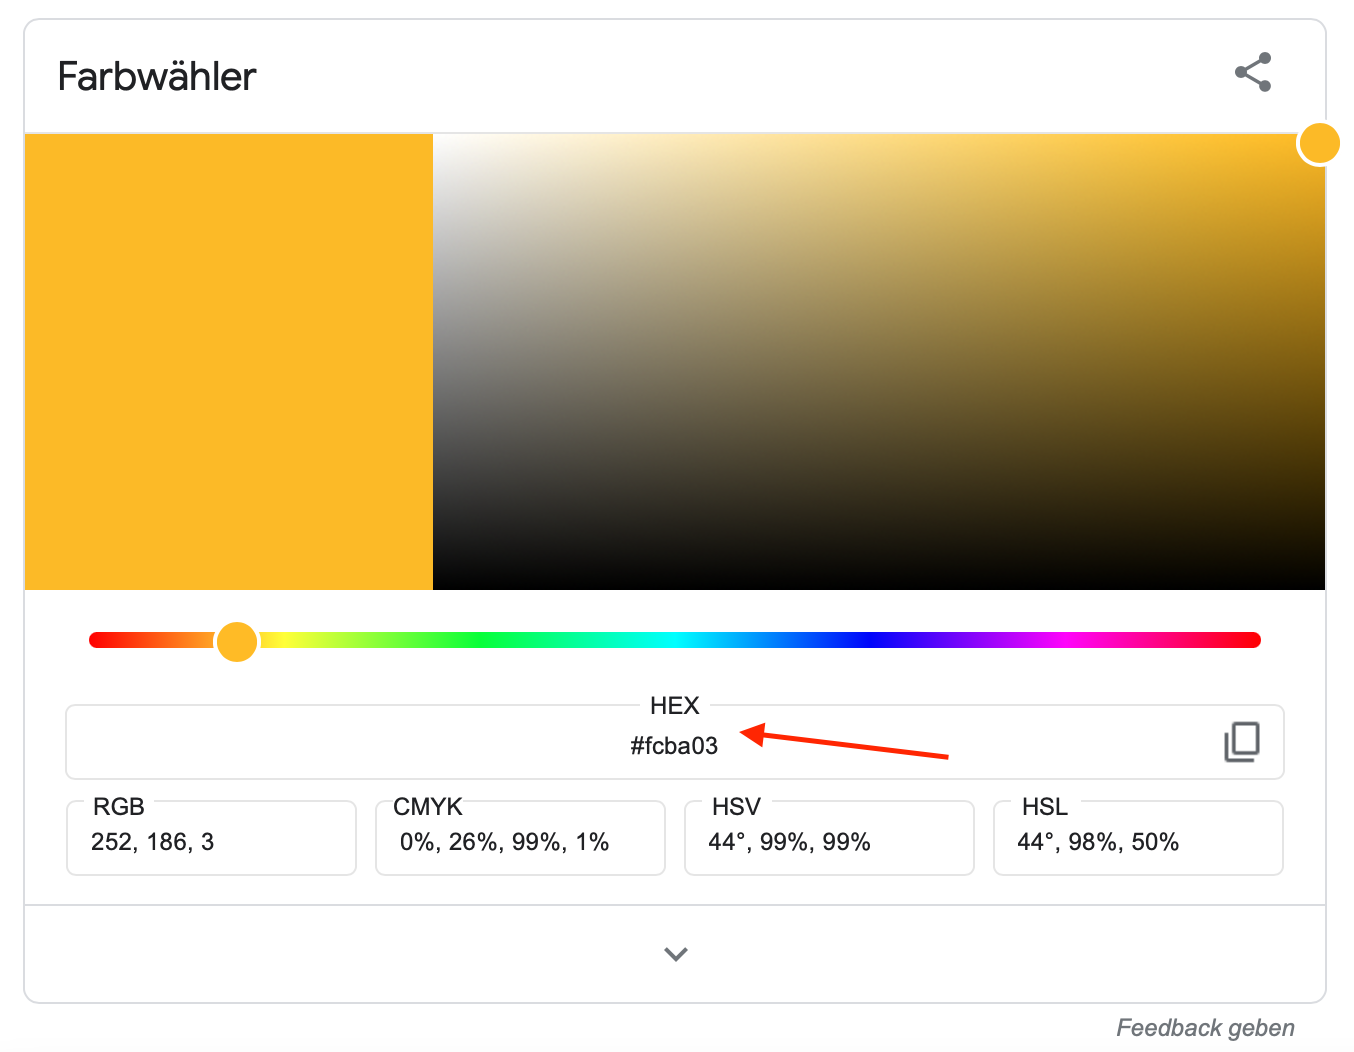
\includegraphics[height=2.5cm]{color_picker}
\caption{Farbwähler von Google.}
\label{figure-color-picker}
\end{minipage}
\end{figure}

\begin{example}[Farbauswahl]
Bildbearbeitungsprogramme geben Farben gerne als Hexadezimalcode an. \autoref{figure-color-picker} zeigt einen Farbwähler (eng. color picker) von Google. Diese Art von Farbangaben finden wir auch beim Erstellen von Websites.
\end{example}

\section{Hexcode, Bits und Bytes}

Eine Hexziffer repräsentiert \qty{4}{\bit}. Wir können somit \qty{1}{\byte} kompakt darstellen. Es benötigt \num{2} Hexziffern. Die grösste Zahl mit zwei Ziffern ist somit $FF_{16}$. Dies entspricht $11111111_2 (= 255_{10})$.

\section{Codieren: Hexzahl $\Rightarrow$ Dualzahl}

Nun geht es darum, wie wir systematisch eine Hexzahl in eine Dualzahl umwandeln. Eine Hexzahl ist der typische Begriff für eine Kombination von Hexadezimalzeichen.

\begin{example}

Wir wandeln die Hexzahl $AB15_{16}$ in eine Dualzahl um.

\begin{center}
$A_{16} = 1010$, $B_{16} = 1011$, $1_{16} = 0001$, $5_{16} = 0101$
\end{center}

Wir erhalten die Dualzahl $1010101100010101_{2}$.

\end{example}

\textbf{Rechenweg:} Wir können von links nach rechts jede Hexadezimalziffer gemäss \autoref{table-hex} bestimmen. Pro Hexadezimalziffer ergibt sich eine vierstellige Dualzahl. Wir notieren die entsprechenden Binärziffern von links nach rechts hintereinander und erhalten die entsprechende Dualzahl.

\subsection{Aufgaben}
\label{subsection-hex2dual-aufgaben}

Wandeln Sie die folgenden Hexadezimalzahlen in die entsprechenden Dualzahlen um. Benutzen Sie \autoref{table-hex-dual}.

\begin{table}[htb]
\centering
\resizebox{\textwidth}{!}{
\begin{tabular}{|c||c|c|c|c|c|c|c|c|c|c|c|c|c|c|c|c|}
\hline
\textbf{Hex}  & 0    & 1    & 2    & 3    & 4    & 5    & 6    & 7    & 8    & 9    & A    & B    & C    & D    & E    & F    \\ \hline
\textbf{Dual} & 0000 & 0001 & 0010 & 0011 & 0100 & 0101 & 0110 & 0111 & 1000 & 1001 & 1010 & 1011 & 1100 & 1101 & 1110 & 1111 \\ \hline
\end{tabular}
}
\caption{Codierungen der Hexadezimalzahlen in den Dualcode.}
\label{table-hex-dual}
\end{table}

\begin{enumerate}
\item $CD_{16}$
\fillwithgrid{0.25in}
\item $101_{16}$
\fillwithgrid{0.25in}
\item $1337_{16}$
\fillwithgrid{0.25in}
\item $CAFE_{16}$
\fillwithgrid{0.25in}
\item $ABBA_{16}$
\fillwithgrid{0.25in}
\item $FFFF_{16}$
\fillwithgrid{0.25in}
\item Wie viel \textbf{Bits} und wie viele \textbf{Bytes} benötigt eine Hexadezimalzahl mit \num{10} Zeichen. Notieren Sie Ihren Rechenweg.
\fillwithgrid{1in}
\end{enumerate}

\section{Decodieren: Dualzahl $\Rightarrow$ Hexzahl}

Nun geht es darum, wie wir systematisch eine Dualzahl in eine Hexzahl umwandeln.

\begin{example}

Wir wandeln die Dualzahl $01111010101100_{2}$ in eine Hexzahl um.

\begin{center}
$01~1110~1010~1100_{2} = 0001~1110~1010~1100_{2} = \underbrace{0001}_{1}~\underbrace{1110}_{E}~\underbrace{1010}_{A}~\underbrace{1100}_{C}$
\end{center}

Wir erhalten die Hexadezimalzahl $1EAC_{16}$.

\end{example}

\textbf{Rechenweg:} Wir bilden von \textbf{rechts} nach \textbf{links} $4$-er Gruppen. Falls die letzte Gruppe \textbf{nicht} aus vier Binärziffern besteht, dann füllen wir diese mit Nullen auf. Wir können dann von \textbf{links} nach \textbf{rechts} jede Hexadezimalziffer gemäss \autoref{table-hex} bestimmen.

\subsection{Aufgaben}
\label{subsection-dual2hex-aufgaben}

Wandeln Sie die folgenden Dualzahlen in die entsprechenden Hexadezimalzahlen um.

\begin{enumerate}
\item $100001_{2}$
\fillwithgrid{0.25in}
\item $11111111_{2}$
\fillwithgrid{0.25in}
\item $1010101010_{2}$
\fillwithgrid{0.25in}
\item $11110000_{2}$
\fillwithgrid{0.25in}
\end{enumerate}

\section{Codieren: Dezimalzahl $\Rightarrow$ Hexzahl}

Nun geht es darum, wie man systematisch eine beliebige, natürliche Zahl aus dem Dezimalsystem in eine Hexzahl umwandeln kann.

\begin{example}
Wir wandeln die Zahl $123\,123_{10}$ in eine Hexzahl um.\\

\begin{minipage}[c][4cm]{0.3\linewidth}
\begin{alignat*}{6}
123\,123 & : & ~16 & ~=~ & 7\,695 & ~R~ & 3 \tikzmark{firstDigitHex} \\
7\,695 & : & ~16 & ~=~ & 480 & ~R~ & F \\
480 & : & ~16 & ~=~ & 30 & ~R~ & 0 \\
30 & : & ~16 & ~=~ & 1 & ~R~ & E \\ 
1 & : & ~16 & ~=~ & 0 & ~R~ & 1 \tikzmark{lastDigitHex} \\
\end{alignat*}
\end{minipage}
\hfill
\begin{minipage}[c][4cm]{0.6\linewidth}
\textbf{Rechenweg:}
\begin{enumerate}
\item Dividieren mit Rest: Dezimalzahl durch 16 teilen und den Rest notieren.
\item Wiederhole die Division mit dem Ergebnis, solange bis das Ergebnis $0$ ist.
\item Lies das Ergebnis ab. Die Hexadezimalziffern für die Hexadezimalzahl sind die Reste von unten nach oben gelesen.
\end{enumerate}
\end{minipage}

\tikz[remember picture] \draw[overlay, ->] ([xshift = 0.5cm]pic cs:lastDigitHex) -- ([xshift = 0.5cm]pic cs:firstDigitHex);

Wir erhalten die Hexadezimalzahl in dem wir die \say{Reste} (Hexadezimalziffern) von \say{unten} nach \say{oben} notieren. Im Beispiel ist dies $1E0F3_{16} = 123\,123_{10}$.

\end{example}

\begin{hinweis}
Bei der Division mit 16 notieren wir den Rest direkt als Hexcode. Im Beispiel ergibt $7\,695 : 16$ den Rest $15_{10}$. Im Hexcode entspricht dies $F_{15}
$.
\end{hinweis}

\subsection{Aufgaben}
\label{subsection-dez2hex-aufgaben}

Wandeln Sie die folgenden dezimalen Zahlen in die entsprechenden Hexadezimalzahlen um. Stellen Sie die Rechenschritte sauber dar.

\begin{enumerate}
\item $93_{10}$
\fillwithgrid{1.25in}
\item $186_{10}$
\fillwithgrid{1.25in}
\item $317_{10}$
\fillwithgrid{1.25in}
\item $\num{642}_{10}$
\fillwithgrid{1.5in}
\item $\num{1025}_{10}$
\fillwithgrid{1.5in}
\end{enumerate}

\section{Decodieren: Hexzahl $\Rightarrow$ Dezimalzahl}

Nun geht es darum, wie man systematisch eine Hexadezimalzahl in eine Dezimalzahl umwandelt.

\begin{example}
Wir wandeln die Zahl $AE17{16}$ in das Dezimalsystem um. Notiere unter die Hexadezimalziffern die $16$-er Potenzen. Beginne bei der Stelle mit dem niedrigsten Stellenwert mit $1$. Multipliziere pro Stelle die Zahl mit $16$. Multipliziere die $16$-er Potenzen mit den Hexadezimalziffern. Addiere abschliessend die individuellen Stellen.

\begin{table}[htb]
\centering
\begin{tabular}{|r|r|r|r|}
\hline
A  & E  & 1  & 7 \\ \hline
$16^3 = 4\,096$  & $16^2 = 256$  & $16^1 = 16$  & $16^0 = 1$ \\ \hline
$A \cdot 4\,096$ & $E \cdot 256$ & $1 \cdot 16$  & $7 \cdot 1$  \\ \hline
$10 \cdot 4\,096$ & $14 \cdot 256$ & $1 \cdot 16$  & $7 \cdot 1$  \\ \hline\hline
40.960 & 3.584 & 16 & 7 \\ \hline
\end{tabular}
\end{table}

$\Rightarrow 7 + 16 + 3\,584 + 40\,960 = 44\,567_{10}$

\end{example}

\subsection{Aufgaben}
\label{subsection-hex2dez-aufgaben}

Wandeln Sie die folgenden Hexadezimalzahlen in die entsprechenden dezimalen Zahlen um. Stellen Sie die Rechenschritte sauber dar.

\begin{enumerate}
\item $73_{16}$
\fillwithgrid{1.25in}
\item $EA_{16}$
\fillwithgrid{1.25in}
\item $1C8_{16}$
\fillwithgrid{1.25in}
\item $15F_{16}$
\fillwithgrid{1.25in}
\item $A09_{16}$
\fillwithgrid{1.25in}
\item $FFF_{16}$
\fillwithgrid{1.25in}
\item $AFFE_{16}$
\fillwithgrid{1.25in}
\end{enumerate}

